\documentclass[conference]{IEEEtran}
\pagestyle{plain}
\usepackage[pdftex]{graphicx}
\graphicspath{{../pdf/}{../jpeg/}}
\DeclareGraphicsExtensions{.pdf,.jpeg,.png}
\usepackage{changepage}
\usepackage[utf8]{inputenc}
\usepackage[T1]{fontenc}
\usepackage{matlab-prettifier}
\usepackage{circuitikz, siunitx}
\usepackage[cmex10]{amsmath}
\usepackage{mathabx}
\usepackage{algorithmic}
\usepackage{float}
\usepackage{array}
\usepackage{mdwmath}
\usepackage{mdwtab}
\usepackage{eqparbox}
\usepackage{url}
\usepackage{makecell}
\usepackage{tikz}
\usepackage{xcolor}
\usepackage{pgfplots}
\IEEEoverridecommandlockouts
\IEEEpeerreviewmaketitle

\pgfplotsset{compat=1.18} 
\usetikzlibrary{shapes.geometric, arrows, arrows.meta, positioning, patterns}

\tikzstyle{startstop} = [rectangle, rounded corners, 
minimum width=3cm, 
minimum height=1cm,
text centered, 
draw=black]

\tikzstyle{io} = [trapezium, 
trapezium stretches=true,
trapezium left angle=70, 
trapezium right angle=110, 
minimum width=3cm, 
minimum height=1cm, text centered, 
draw=black]

\tikzstyle{process} = [rectangle, 
minimum width=3cm, 
minimum height=1cm, 
text centered, 
text width=3cm, 
draw=black]

\tikzstyle{decision} = [diamond, 
minimum width=3cm, 
minimum height=1cm, 
text centered, 
draw=black]

\tikzstyle{arrow} = [thick,->,>=stealth]
\tikzstyle{invarrow} = [thick,<-,>=stealth]
        
\begin{document}

\title{Sistema Automatizado de Clasificación e Inspección de Calidad Multivariable Basado en Sensores Industriales y Arquitectura Concurrente ESP32-Python\\ {\huge Automated Multivariable Sorting and Quality Inspection System Based on Industrial Sensors and ESP32-Python Concurrent Architecture}}

\author{
    \authorblockN{
        M. Rodríguez \\
    }
    \authorblockA{
        \textit{Universidad de los Llanos} \\
        \textit{Villavicencio, Colombia} \\ 
        {\small \texttt{marodriguez.payares@unillanos.edu.co 161004834}}
    }
}
\IEEEaftertitletext{\vspace{-1\baselineskip}}
\maketitle

\renewcommand\abstractname{Resumen}
\begin{abstract}
El presente informe detalla el diseño, caracterizacion e implementacion de un prototipo automatizado para la clasificacion y conteo de objetos en una linea de produccion en tiempo real. La arquitectura de hardware propuesta integra coordinadamente tres transductores de grado industrial de distinta naturaleza fisica: un sensor fotoelectrico  BMS2M-MDT como contador maestro, un sensor inductivo PR12-4DN para la identificacion de elementos metalicos y un sensor capacitivo CR18-8DN enfocado en el control de calidad de fluidos \cite{sensores_3, sensores_14}. Las señales NPN de colector abierto fueron acondicionadas de manera segura hacia un microcontrolador ESP32 utilizando las resistencias de pull-up internas, donde se procesaron mediante rutinas de interrupcion externa (ISR) y un algoritmo de filtrado temporal (debounce) de 300 ms. Para la visualizacion de datos, se desarrollo una interfaz grafica de usuario (HMI) en Python que implementa programacion concurrente (\textit{multithreading}), aislando la lectura del puerto serial del bucle de refresco de la GUI \cite{sensores_20}. Los resultados experimentales validaron la robustez del sistema con una precision superior al 95\% en el conteo general y una eficiencia del 100\% en la deteccion de metales. Asimismo, se demostro la selectividad dielectrica del transductor capacitivo, el cual logro discriminar la alta constante dielectrica del agua ($\varepsilon_r \approx 80$) frente a la firma del aire y del polietileno ($\varepsilon_r \approx 1-3$), bloqueando falsos positivos y rechazando el 100\% de los envases vacios \cite{sensores_16}. Finalmente, el analisis critico identifico las limitaciones de rango operativo y el crosstalk estructural, sentando las bases para futuras mejoras mediante control PID y protocolos de comunicacion orientados a la Industria 4.0.
\end{abstract}

\renewcommand\IEEEkeywordsname{Palabras clave}
\begin{keywords}
Control de calidad, discriminacion dielectrica, interrupciones en tiempo real, programacion concurrente, sensores industriales.
\end{keywords}

\renewcommand\abstractname{Abstract}
\begin{abstract}
This report details the design, characterization, and implementation of an automated prototype for real-time object sorting and counting on a production line. The proposed hardware architecture coordinately integrates three industrial-grade transducers of different physical natures: a  BMS2M-MDT photoelectric sensor as a master counter, a PR12-4DN inductive sensor for identifying metallic elements, and a CR18-8DN capacitive sensor focused on fluid quality control \cite{sensores_3, sensores_14}. The open-collector NPN signals were safely conditioned to an ESP32 microcontroller using internal pull-up resistors, where they were processed via external interrupt service routines (ISR) and a 300 ms temporal filtering (debounce) algorithm. For data visualization, a graphical user interface (GUI) was developed in Python implementing concurrent programming (multithreading), isolating the serial port reading from the GUI refresh loop \cite{sensores_20}. Experimental results validated the system's robustness with an overall counting accuracy exceeding 95\% and a 100\% efficiency in metal detection. Furthermore, the dielectric selectivity of the capacitive transducer was demonstrated, successfully discriminating the high dielectric constant of water ($\varepsilon_r \approx 80$) against the signature of air and polyethylene ($\varepsilon_r \approx 1-3$), effectively blocking false positives and rejecting 100\% of the empty containers \cite{sensores_16}. Finally, a critical analysis identified operational range limitations and structural crosstalk, laying the groundwork for future improvements through PID control and Industry 4.0 oriented communication protocols.
\end{abstract}

\renewcommand\IEEEkeywordsname{Keywords}
\begin{keywords}
Concurrent programming, dielectric discrimination, industrial sensors, quality control, real-time interrupts.
\end{keywords}

\section{Introducción}

La evolución de los entornos productivos hacia la fabrica inteligente ha sido impulsada por la necesidad de optimizar la precisión y la velocidad en las lineas de montaje. En este contexto, la contextualización de la automatización industrial revela que el reemplazo de tareas manuales de conteo y clasificación por sistemas automaticos ha permitido mitigar el error humano, el cual es inherente a la fatiga y a la naturaleza repetitiva de estas labores \cite{sensores_1}. La implementación de estaciones de trabajo capaces de procesar información en tiempo real no solo incrementa la eficiencia operativa, sino que también garantiza una trazabilidad mas rigurosa de los insumos y productos terminados, permitiendo una integracion fluida con sistemas de control jerárquicos y de gestión de materiales \cite{sensores_2}.

Un aspecto critico en el diseño de estos sistemas es la importancia de la selección de sensores según la naturaleza del objeto. En el ámbito de la automatización, no existe un dispositivo de detección universal que pueda identificar todas las variables de un proceso con la misma eficacia \cite{sensores_11}. Por el contrario, la selección tecnológica debe fundamentarse en las propiedades físicas especificas de la carga o el material que se pretende supervisar, ya sean estas propiedades ópticas, ferromagnéticas o dieléctricas \cite{sensores_3}.

Para la detección general de objetos en una cinta transportadora, se recurre a la tecnología fotoeléctrica, la cual aprovecha las propiedades ópticas de los materiales para interrumpir o reflejar un haz de luz, permitiendo un conteo versátil sin contacto físico \cite{sensores_7, sensores_9}. Sin embargo, cuando el requerimiento exige la discriminación de piezas metálicas entre una diversidad de materiales, se hace necesario el uso de sensores inductivos. Estos dispositivos operan bajo el principio de corrientes de Eddy y variaciones de flujo magnético, interactuando específicamente con las propiedades ferromagnéticas de los metales \cite{sensores_4, sensores_19}.

Finalmente, para aplicaciones mas complejas donde se requiere detectar la presencia de líquidos o el nivel de llenado dentro de un recipiente, la selección se desplaza hacia el sensado capacitivo. Esta tecnología es sensible a las variaciones en las propiedades dieléctricas del medio, lo que permite al sensor CR18-8DN distinguir entre una botella vacía y una llena de agua debido al cambio significativo en la capacitancia del sistema \cite{sensores_16, sensores_18}. Así, la integración de estos tres principios de funcionamiento asegura una caracterización completa del flujo de producción, adaptándose a la versatilidad requerida por las exigencias industriales modernas \cite{sensores_14}.

\subsection{Justificación del Sistema de Detección Multivariable}

El diseño especifico de esta arquitectura de sensado se fundamenta en la necesidad de un control integral y selectivo de la producción. Tras analizar los requerimientos del entorno y el comportamiento de cada variable, se ha asignado un rol determinístico a cada uno de los tres sensores, aprovechando sus principios físicos individuales explicados a continuación.

El sensor fotoeléctrico  BMS2M-MDT ejerce la función de contador maestro del sistema y opera bajo el principio óptico retro-reflectivo. Como se observa en la Figura \ref{fig:principio_foto}, el emisor y el receptor se encuentran alojados en el mismo encapsulado. El emisor proyecta un haz de luz con una intensidad inicial hacia un reflector externo, el cual devuelve la señal al receptor; la detección se produce cuando un objeto opaco se interpone en este trayecto, interrumpiendo el flujo luminoso \cite{sensores_11, sensores_9}. Este fenómeno de absorción y bloqueo obedece a la ley de atenuación, modelada por la ecuación:
\begin{equation}
    I = I_0 e^{-\alpha x}
\end{equation}

\begin{figure}[htbp]
    \centering
    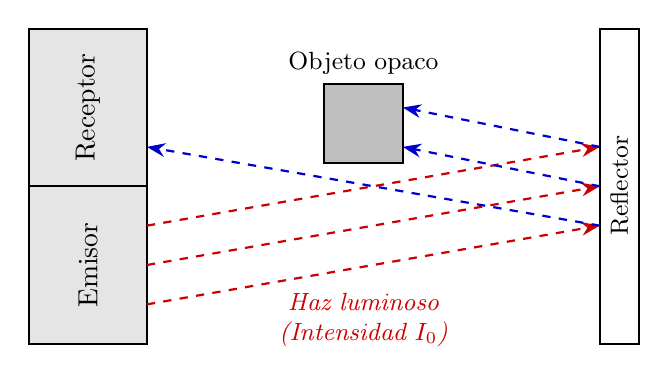
\begin{tikzpicture}[
        node distance = 1cm and 2cm,
        sensor/.style={fill=gray!20, draw=black, thick, minimum width=1.5cm, minimum height=2cm},
        beam1/.style={->, >=Stealth, red!80!black, thick, dashed},
        beam2/.style={->, >=Stealth, blue!80!black, thick, dashed},
    ]
        \node[sensor] (emisor) at (-3.5,0) {\rotatebox{90}{Emisor}};
        \node[sensor] (receptor) at (-3.5,2) {\rotatebox{90}{Receptor}};
        \draw[fill=white!50, draw=black, thick] (3.5,3) rectangle (3,-1);
        \node[anchor=south, font=\small, color=black] at (3.25,0.25) {\rotatebox{90}{Reflector}};

        \draw[fill=gray!50, draw=black, thick] (-0.5,1.3) rectangle (0.5,2.3);
        \node[anchor=south, font=\small, color=black] at (0,2.3) {Objeto opaco};
        
        \draw[beam1] (-2.75, -0.5) -- (3, 0.5);
        \draw[beam1] (-2.75, 0) -- (3, 1);
        \draw[beam1] (-2.75, 0.5) -- (3, 1.5);

        \draw[beam2] (3, 0.5) -- (-2.75, 1.5);
        \draw[beam2] (3, 1) -- (0.5, 1.5);
        \draw[beam2] (3, 1.5) -- (0.5, 2);
        
        \node[text width=2.5cm, align=center, font=\small\itshape, color=red!80!black] at (0, -0.7) {
            Haz luminoso\\
            (Intensidad $I_0$)
        };
    \end{tikzpicture}
    \caption{Esquema del principio físico de interrupción óptica en el sensor fotoeléctrico BMS2M-MDT.}
    \label{fig:principio_foto}
\end{figure}

donde $I$ representa la intensidad luminosa final que llega al receptor, $I_0$ es la intensidad emitida, $\alpha$ es el coeficiente de atenuación del obstáculo y $x$ es el espesor del material \cite{sensores_17}. Para asegurar un conteo preciso sin falsos positivos, la Figura \ref{fig:respuesta_foto} expone la curva característica del área de sensado en función de la distancia de detección. Esta gráfica delimita un perfil espacial de forma parabólica que define la zona de operación óptica estable, fuera de la cual el sensor ignora perturbaciones \cite{sensores_15}.

\begin{figure}[htbp]
    \centering
    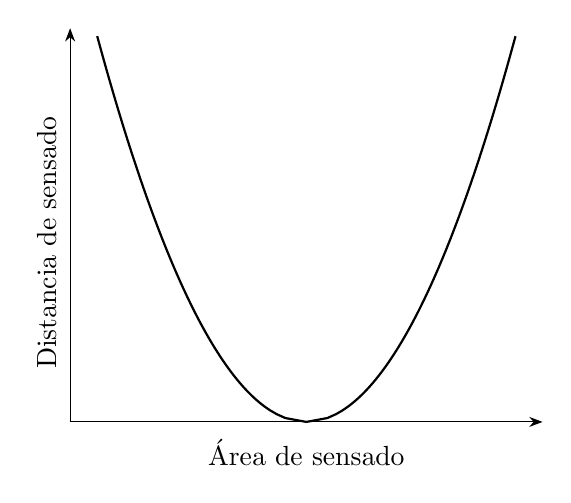
\begin{tikzpicture}[scale=1]
        \draw[->, >=Stealth] (-3,0) -- (3,0) node[midway, anchor=north, yshift=-0.1cm] {Área de sensado};
        \draw[->, >=Stealth] (-3,0) -- (-3,5) node[rotate=90, anchor=east, yshift=0.3cm, xshift=-1cm] {Distancia de sensado};
        
        \draw[thick, black, domain=0.0:4.9, samples=100] 
            plot ({1.2*sqrt(\x)}, \x)
            plot ({-1.2*sqrt(\x)}, \x);
    \end{tikzpicture}
    \caption{Diagrama del área de operación del sensor fotoeléctrico: ancho del haz de detección en función de la distancia de sensado.}
    \label{fig:respuesta_foto}
\end{figure}

Por su parte, el sensor inductivo PR12-4DN se implementa para la discriminación especifica de elementos metálicos \cite{sensores_5}. Su principio de funcionamiento, ilustrado en la Figura \ref{fig:principio_inductivo}, se basa en la inducción electromagnética. Una bobina osciladora interna genera un campo magnético de alta frecuencia en la cara activa del sensor. Cuando un material ferromagnético o conductor ingresa a este campo, se inducen corrientes de Eddy (o corrientes de Foucault) en la superficie del objeto, las cuales absorben energía y atenúan la amplitud del circuito oscilador \cite{sensores_19}. Este cambio fisico altera la inductancia del circuito, regida por la ecuación:
\begin{equation}
    L = \frac{N^2}{\mathcal{R}}
\end{equation}

\begin{figure}[htbp]
    \centering
    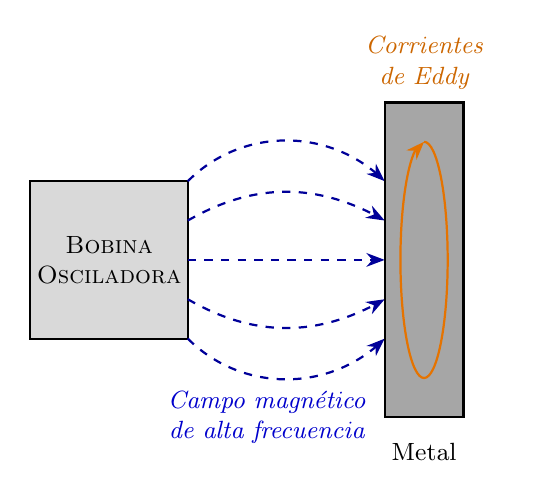
\begin{tikzpicture}[
        node distance = 1cm and 2cm,
        sensor/.style={fill=gray!30, draw=black, thick},
        field/.style={->, >=Stealth, blue!60!black, thick, dashed},
        eddy/.style={->, >=Stealth, orange!90!black, thick},
    ]
        \draw[sensor] (-3, -1) rectangle (-1, 1);
        \node[font=\small\scshape, align=center] at (-2, 0) {Bobina\\Osciladora};
        
        \draw[field] (-1, 1) to[bend left=45] (1.5, 1);
        \draw[field] (-1, 0.5) to[bend left=30] (1.5, 0.5);
        \draw[field] (-1, 0) -- (1.5, 0);
        \draw[field] (-1, -0.5) to[bend right=30] (1.5, -0.5);
        \draw[field] (-1, -1) to[bend right=45] (1.5, -1);
        
        \draw[fill=gray!70, draw=black, thick] (1.5, -2) rectangle (2.5, 2);
        \node[anchor=north, font=\small, color=black] at (2, -2.2) {Metal};

        \draw[eddy] (2, 1.5) arc (90:-270:0.3 and 1.5);
        
        \node[text width=3cm, align=center, font=\small\itshape, color=blue!80!black] at (0, -2) {
            Campo magnético\\
            de alta frecuencia
        };
        \node[text width=2.5cm, align=center, font=\small\itshape, color=orange!80!black] at (2, 2.5) {
            Corrientes\\
            de Eddy
        };
    \end{tikzpicture}
    \caption{Principio de inducción electromagnética y generación de corrientes de Foucault en el sensor PR12-4DN.}
    \label{fig:principio_inductivo}
\end{figure}

siendo $N$ el numero de espiras de la bobina y $\mathcal{R}$ la reluctancia del circuito magnético \cite{sensores_4}. La Figura \ref{fig:respuesta_inductivo} describe la relación directa entre el tamaño del objeto metálico y la distancia de detección relativa ($S_r$). Como se evidencia en la curva exponencial, para lograr el cien por ciento de la distancia nominal de sensado, el objeto metálico debe alcanzar un tamaño o área frontal especifica; objetos mas pequeños reducirán la capacidad de detección \cite{sensores_8}.

\begin{figure}[htbp]
    \centering
    \begin{tikzpicture}[scale=1]
        \draw[->, >=Stealth] (0,0) -- (6,0) node[midway, anchor=north, yshift=-0.1cm] {Tamaño del objeto};
        \draw[->, >=Stealth] (0,0) -- (0,5) node[rotate=90, anchor=east, yshift=0.3cm, xshift=-2cm] {Sr (\%)};
        
        \draw[thick, black, domain=0:5.8, samples=100] 
            plot (\x, {4.5*(1 - exp(-1.5*\x))});
            
    \end{tikzpicture}
    \caption{Relación entre el tamaño del objeto y la distancia de detección relativa ($S_r$) de un sensor inductivo.}
    \label{fig:respuesta_inductivo}
\end{figure}

Finalmente, el sensor capacitivo CR18-8DN actúa como un instrumento de control de calidad, configurado para discriminar botellas de agua llenas de las vacías \cite{sensores_16}. Como detalla la Figura \ref{fig:principio_capacitivo}, los electrodos concéntricos del sensor generan un campo eléctrico que penetra la pared del envase plástico. El principio físico aprovecha el hecho de que el agua posee una constante dieléctrica ($\varepsilon_r \approx 80$) significativamente mayor a la del plástico ($\varepsilon_r \approx 2$) y del aire. La capacitancia del sistema responde a la ecuación:
\begin{equation}
    C = \frac{\varepsilon_0 \varepsilon_r A}{d}
\end{equation}

\begin{figure}[htbp]
    \centering
    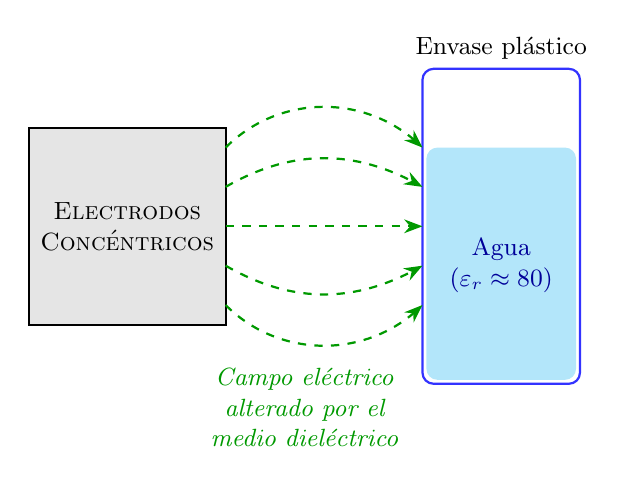
\begin{tikzpicture}[
        node distance = 1cm and 2cm,
        sensor/.style={fill=gray!20, draw=black, thick},
        efield/.style={->, >=Stealth, green!60!black, thick, dashed},
    ]
        \draw[sensor] (-3.5, -1.25) rectangle (-1, 1.25);
        \node[font=\small\scshape, align=center] at (-2.25, 0) {Electrodos\\Concéntricos};

        \draw[draw=blue!80, thick, rounded corners] (1.5, -2) rectangle (3.5, 2);
        \node[anchor=south, font=\small, color=black] at (2.5, 2) {Envase plástico};

        \fill[cyan!30, rounded corners] (1.55, -1.95) rectangle (3.45, 1);
        \node[font=\small, color=blue!60!black, align=center] at (2.5, -0.5){Agua\\($\varepsilon_r \approx 80$)};

        \draw[efield] (-1, 1) to[bend left=45] (1.5, 1);
        \draw[efield] (-1, 0.5) to[bend left=30] (1.5, 0.5);
        \draw[efield] (-1, 0) -- (1.5, 0);
        \draw[efield] (-1, -0.5) to[bend right=30] (1.5, -0.5);
        \draw[efield] (-1, -1) to[bend right=45] (1.5, -1);

        \node[text width=3.5cm, align=center, font=\small\itshape, color=green!60!black] at (0, -2.3) {
            Campo eléctrico\\
            alterado por el\\
            medio dieléctrico
        };
    \end{tikzpicture}
    \caption{Interacción del campo eléctrico del sensor capacitivo CR18-8DN con un medio de alta permitividad (agua).}
    \label{fig:principio_capacitivo}
\end{figure}

donde $\varepsilon_0$ es la permitividad del vacío, $\varepsilon_r$ la permitividad relativa del material interactuando con el campo, $A$ el área de los electrodos y $d$ la distancia de separación \cite{sensores_6}. La Figura \ref{fig:respuesta_capacitivo} ilustra la curva caracteristica que vincula la constante dieléctrica del material con la distancia de detección relativa ($S_r$). Se observa que un material con alta permitividad (como el agua) incrementa la distancia efectiva, lo que permite calibrar el umbral del sensor para que conmute unicamente al detectar el liquido y permanezca inactivo ante un envase vacío \cite{sensores_18, sensores_20}.

\begin{figure}[htbp]
    \centering
    \begin{tikzpicture}[scale=1]
        \draw[->, >=Stealth] (0,0) -- (6,0) node[midway, anchor=north, yshift=-0.1cm] {Sr (\%)};
        \draw[->, >=Stealth] (0,0) -- (0,5) node[rotate=90, anchor=east, yshift=0.3cm, xshift=-0.7cm] {Constante dieléctrica ($\epsilon_r$)};
        \draw[thick, black, domain=0.1:5.9, samples=100] 
            plot (\x, {0.15*\x + 0.0005*exp(1.5*\x)});
    \end{tikzpicture}
    \caption{Curva de respuesta típica de un sensor capacitivo: relación entre la constante dieléctrica del material y la distancia de detección nominal.}
    \label{fig:respuesta_capacitivo}
\end{figure}

\subsection{Definición del Problema: Discriminación de Estados de Llenado}

Uno de los retos críticos en las líneas de envasado automatizadas es la detección no invasiva del contenido líquido. La problemática técnica radica en diferenciar con precisión una botella llena de una vacía sin comprometer la integridad del empaque ni ralentizar el flujo de producción. 

Desde la perspectiva del sensado industrial, un envase plástico vacío y uno lleno presentan una geometría exterior idéntica, lo que anula la eficacia de sensores de proximidad mecánicos o inductivos. El desafío se resuelve mediante la explotación de las propiedades dieléctricas de los materiales involucrados. Mientras que el polímero del envase posee una constante dieléctrica baja ($\varepsilon_r \approx 2$ a $3$), el agua presenta una permitividad relativa excepcionalmente alta ($\varepsilon_r \approx 80$). 

El problema se aborda calibrando el sensor capacitivo CR18-8DN para que el incremento de capacitancia provocado únicamente por la pared del plástico sea insuficiente para alcanzar el umbral de conmutación. Solo cuando el campo eléctrico interactúa con la masa de agua interior, la capacitancia total del sistema aumenta lo suficiente según la ecuación $C = \frac{\varepsilon_0 \varepsilon_r A}{d}$, permitiendo una clasificación binaria (Lleno/Vacío) en tiempo real.

El presente documento se encuentra organizado de la siguiente manera: en la sección de Metodología se describe el montaje experimental y la lógica de programación del firmware; posteriormente, en la sección de Resultados, se analizan las curvas de respuesta obtenidas y la eficiencia del conteo multivariable; finalmente, se presentan las Conclusiones y recomendaciones técnicas para la optimización de sistemas de clasificación industrial.

\section{Materiales y Métodos}

\subsection{Especificaciones de los Dispositivos de Sensado}

Para la implementación del prototipo de clasificación y conteo, se seleccionaron tres sensores de grado industrial, cada uno destinado a evaluar una caracteristica física especifica de los objetos en la linea de prueba \cite{sensores_3}. La integración concurrente de estos dispositivos requiere una comprensión precisa de sus parámetros eléctricos y de sus limites de detección espaciales para garantizar una interfaz adecuada y segura con la etapa de procesamiento digital \cite{sensores_14}. 

En la Tabla \ref{tab:especificaciones_sensores} se resumen las características operativas fundamentales de los tres dispositivos analizados: el sensor fotoeléctrico  BMS2M-MDT utilizado para el conteo global \cite{sensores_11}, el sensor inductivo PR12-4DN especifico para metales \cite{sensores_5} y el sensor capacitivo CR18-8DN destinado a la detección de fluidos \cite{sensores_16}. 

Es imperativo destacar que los tres sensores operan en un rango de alimentación estándar para tableros de control industrial (12 a 24 V DC) y comparten una arquitectura de conmutación basada en un transistor NPN de colector abierto. Esta configuración de salida resulta altamente ventajosa para el diseño del circuito, dado que, al no suministrar voltaje activamente por la linea de señal, permite adaptar los niveles de tensión a los 3.3 V requeridos por los pines GPIO del microcontrolador mediante el uso de resistencias de pull-up, protegiendo así la integridad del sistema embebido.

\begin{table*}[htbp]
    \centering
    \caption{Especificaciones técnicas operativas de los sensores industriales implementados en el sistema de clasificación.}
    \label{tab:especificaciones_sensores}
    \begin{tabular}{lccc}
        \hline
        Parámetro de operación & Fotoeléctrico & Inductivo & Capacitivo \\
        \hline
        Modelo del dispositivo &  BMS2M-MDT & PR12-4DN & CR18-8DN \\
        Configuración de salida & NPN (L-ON / D-ON) & NPN (NO) & NPN (NO) \\
        Distancia de detección nominal & 2 m & 4 mm & 8 mm \\
        Voltaje de alimentación & 12-24 V DC & 12-24 V DC & 12-24 V DC \\
        \hline
    \end{tabular}
\end{table*}

\subsection{Arquitectura de Hardware y Conectividad}

La integridad de los datos en el sistema de conteo depende de una arquitectura de hardware capaz de traducir las señales de conmutación de nivel industrial (24 V DC) a niveles lógicos compatibles con la arquitectura CMOS del microcontrolador ESP32 (3.3 V DC). Al igual que en sistemas de monitoreo de variables ambientales, la robustez frente al ruido eléctrico y la protección de las entradas digitales son pilares fundamentales del diseño \cite{sensores_14}.

\subsubsection{Interfaz de Acoplamiento y Acondicionamiento de señal}
Dado que los sensores seleccionados poseen una etapa de salida tipo NPN de colector abierto, la interfaz de acoplamiento se simplifica significativamente. En esta configuración, el sensor actúa como un interruptor que conmuta la linea de señal a tierra (GND) cuando se activa, dejando la linea en estado de alta impedancia (flotante) cuando esta inactivo. 

Para adaptar esta señal, se implemento una configuración de resistencia de pull-up conectada a la fuente de 3.3 V del ESP32 en cada uno de los pines GPIO ($12$, $13$ y $14$). Esta técnica asegura que el pin de entrada nunca experimente los 24 V de la fuente de alimentación industrial, sino que oscile estrictamente entre $0$ V (estado bajo/activo) y $3.3$ V (estado alto/inactivo), cumpliendo con los requerimientos de la unidad de procesamiento sin necesidad de divisores de tensión complejos o dispositivos de opto-acoplamiento adicionales.

\subsubsection{Diagrama de Conexiones}
Como se ilustra en el esquema circuital de la Figura \ref{fig:diagrama_conexiones}, el sistema utiliza una referencia de tierra común (GND) entre la fuente industrial y el microcontrolador. Esta referencia compartida es critica para cerrar el lazo de corriente del transistor de salida de los sensores y garantizar una detección de flancos estable por parte de las interrupciones externas (ISR) programadas en el firmware.

\begin{figure}[htbp]
    \centering
    \begin{circuitikz}[scale=0.65, transform shape]
        \draw (0,0) node[draw, rectangle, minimum width=4cm, minimum height=10cm, anchor=west, fill=blue!5] (ESP) {ESP32};
        
        \draw (ESP.north) ++(-1,0) node[below] {VCC} to[short] ++(0,0.5) node[vcc]{+3.3V};
        \draw (ESP.north) ++(1,0) node[below] {UART} to[short, -o] ++(0,1) node[above] {PC};
        \draw (ESP.south) node[above] {GND} node[ground]{};
        
        \draw (-5,3.5) node[draw, rectangle, minimum width=2.5cm, minimum height=2cm, fill=gray!10] (S1) {BMS2M};
        \node[above, font=\scriptsize] at (S1.north) {Fotoeléctrico};
       
        \draw (S1.west) ++(0,0.5) -- ++(-0.5,0) node[vcc] {+24V};
        \draw (S1.west) ++(0,-0.5) -- ++(-0.5,0) node[ground] {};
        
        \draw (S1.east) to[short, -o] (0,3.5) node[right] {GPIO 13};
        \draw (-1.5,3.5) to[R, l=$10k\Omega$, *-] ++(0,2) node[vcc] {+3.3V};

        \draw (-5,0) node[draw, rectangle, minimum width=2.5cm, minimum height=2cm, fill=gray!10] (S2) {PR12-4D};
        \node[above, font=\scriptsize] at (S2.north) {Inductivo};

        \draw (S2.west) ++(0,0.5) -- ++(-0.5,0) node[vcc] {+24V};
        \draw (S2.west) ++(0,-0.5) -- ++(-0.5,0) node[ground] {};

        \draw (S2.east) to[short, -o] (0,0) node[right] {GPIO 12};
        \draw (-1.5,0) to[R, l=$10k\Omega$, *-] ++(0,2) node[vcc] {+3.3V};

        \draw (-5,-3.5) node[draw, rectangle, minimum width=2.5cm, minimum height=2cm, fill=gray!10] (S3) {CR18-8D};
        \node[above, font=\scriptsize] at (S3.north) {Capacitivo};

        \draw (S3.west) ++(0,0.5) -- ++(-0.5,0) node[vcc] {+24V};
        \draw (S3.west) ++(0,-0.5) -- ++(-0.5,0) node[ground] {};

        \draw (S3.east) to[short, -o] (0,-3.5) node[right] {GPIO 14};
        \draw (-1.5,-3.5) to[R, l=$10k\Omega$, *-] ++(0,2) node[vcc] {+3.3V};
    \end{circuitikz}
    \caption{Arquitectura de conexionado eléctrico. Se destaca el uso de GND común y la utilización de resistencias de pull-up internas para la adaptación de niveles lógicos NPN.}
    \label{fig:diagrama_conexiones}
\end{figure} 

\subsection{Caracterización y Calibración del Sensor Capacitivo}

La eficacia del sistema de control de calidad reside en la capacidad del sensor CR18-8DN para realizar una discriminación dieléctrica precisa. A diferencia de los sensores inductivos, cuya respuesta es predominantemente binaria ante la presencia de metales, el sensor capacitivo requiere un proceso de caracterización empírica para establecer un umbral de conmutación que ignore el contenedor y detecte exclusivamente el contenido liquido \cite{sensores_16}.

\subsubsection{Procedimiento de Ajuste de Sensibilidad}
El sensor CR18-8DN integra en su parte posterior un potenciómetro de precisión (multivuelta) protegido por una cubierta de polímero, el cual permite desplazar el punto de operación del circuito oscilador interno. El proceso de calibración se realizo siguiendo un protocolo de aproximación sucesiva:
\begin{enumerate}
    \item Se posiciono una botella de polietileno vacía a la distancia nominal de operación ($8$ mm).
    \item Se giro el potenciómetro en sentido antihorario hasta que el indicador LED de estado se apagara por completo, asegurando que la permitividad del aire y del plástico ($\varepsilon_r \approx 2$) no fuera suficiente para alterar el campo eléctrico por encima del umbral de disparo.
    \item Posteriormente, se introdujo una muestra de agua en el envase y se verifico la activación inmediata del sensor. 
    \item Se realizo un ajuste fino girando levemente en sentido horario para maximizar el margen de ruido, garantizando que variaciones menores en el espesor del plástico no generaran falsos positivos.
\end{enumerate}

\subsubsection{Análisis de la Respuesta ante la Permitividad Relativa}
La calibración se fundamenta en la diferencia de magnitudes de la permitividad relativa entre los materiales presentes en la linea. El sensor detecta una capacitancia total $C_{total}$ que es la suma de las contribuciones del aire, el envase y el contenido. Dado que la permitividad del agua ($\varepsilon_r \approx 80$) es aproximadamente $40$ veces superior a la del plástico, el sistema experimenta un incremento súbito en la densidad de flujo eléctrico al detectar el fluido \cite{sensores_18}.

Como se analizo en la sección de principios físicos, este contraste permite que el sensor actúe como un filtro de paso alto para la constante dieléctrica. En las pruebas de laboratorio, se valido que el umbral establecido permitió ignorar no solo el envase vacío, sino también otros materiales con baja permitividad como cartón o madera seca, asegurando que el contador de botellas llenas responda exclusivamente a la variable de interés: la presencia de agua liquida \cite{sensores_20}.

\subsection{Lógica de Discriminación y Algoritmo de Conteo}

El cerebro del sistema se divide en dos etapas de procesamiento: una etapa de tiempo real ejecutada por el microcontrolador para la captura de eventos, y una etapa de visualización y gestión de datos en una estación de trabajo mediante un script de Python. Esta arquitectura garantiza que ningún pulso de detección se pierda debido a latencias en la interfaz gráfica \cite{sensores_14}.

\subsubsection{Manejo de Interrupciones y Algoritmo Anti-rebote (Debounce)}
Para garantizar una respuesta inmediata ante el paso de objetos en la linea de alta velocidad, el firmware desarrollado en el archivo \texttt{sensores.ino} utiliza interrupciones externas asociadas a los pines GPIO $12$, $13$ y $14$. Se configuro el disparo por flanco de bajada (\texttt{FALLING}), dado que los sensores NPN conmutan a un estado lógico bajo al detectar un objetivo.

Un reto técnico identificado fue la presencia de ruido eléctrico y vibraciones mecánicas que generaban múltiples disparos por un solo objeto. Para mitigar esto, se implemento un algoritmo de antirrebote por software mediante la comparación de marcas de tiempo utilizando la función \texttt{millis()}. Como se detalla en el fragmento de código, solo se incrementa el contador si han transcurrido al menos $300$ ms desde el ultimo evento validado:
\begin{equation}
    t_{actual} - t_{ultimo\_evento} > t_{debounce}
\end{equation}
Este filtro temporal asegura que la matriz de decisión procese señales limpias y únicas por cada elemento en transito.

\subsubsection{Flujo de Operación del Firmware}
La lógica del lazo principal del ESP32 se encarga de empaquetar los valores acumulados en las variables volátiles y transmitirlos mediante una trama serial formateada por comas (\texttt{CSV}). El diagrama de flujo de la Figura \ref{fig:flow_ESP32} ilustra esta secuencia lógica simplificada.

\begin{figure}[htbp]
    \centering
    \resizebox{0.7\columnwidth}{!}{
    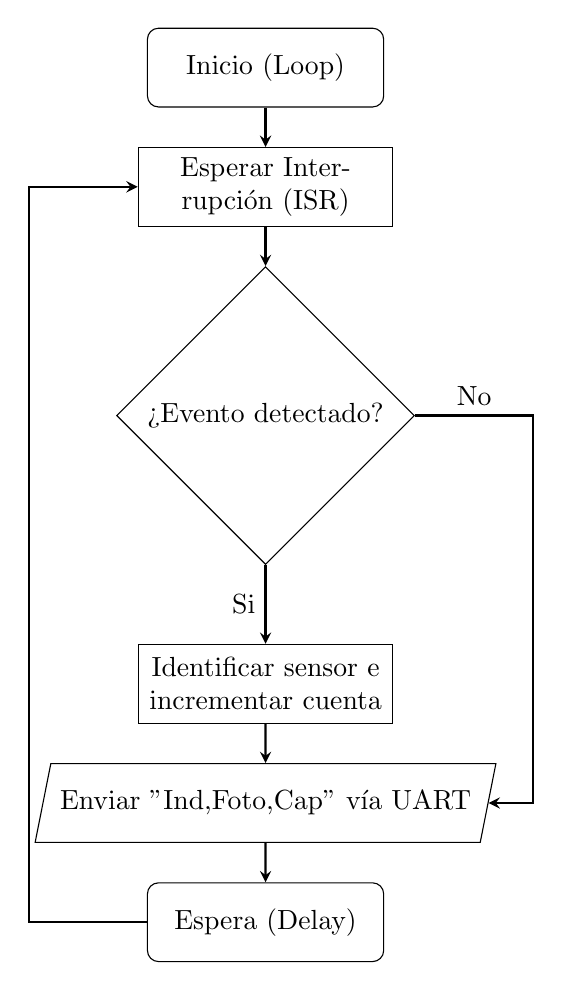
\begin{tikzpicture}[node distance=0.5cm, auto]
        
        \node (start) [startstop] {Inicio (Loop)};
        \node (isr) [process, below=of start] {Esperar Interrupción (ISR)};
        \node (dec_event) [decision, below=of isr] {¿Evento detectado?};
        \node (proc_count) [process, below=of dec_event, yshift=-0.5cm] {Identificar sensor e incrementar cuenta};
        \node (proc_send) [io, below=of proc_count] {Enviar "Ind,Foto,Cap" vía UART};
        \node (stop) [startstop, below=of proc_send] {Espera (Delay)};

        \draw [arrow] (start) -- (isr);
        \draw [arrow] (isr) -- (dec_event);
        \draw [arrow] (dec_event) -- node[anchor=east] {Si} (proc_count);
        \draw [arrow] (proc_count) -- (proc_send);
        \draw [arrow] (proc_send) -- (stop);
        \draw [arrow] (stop.west) -- ++(-1.5,0) |- (isr.west);

        \draw [arrow] (dec_event.east) -- ++(1.5,0) node[midway, above] {No} |- (proc_send.east);

    \end{tikzpicture}
    }
    \caption{Diagrama de flujo del firmware de conteo y discriminación implementado en el ESP32.}
    \label{fig:flow_ESP32}
\end{figure}

\subsubsection{Procesamiento Multihilo y Visualización (Python)}
En la etapa de recepción, el script \texttt{visual.py} implementa un enfoque de programación concurrente (\textit{multithreading}) para gestionar la interfaz gráfica de usuario (GUI). Esta técnica es crucial ya que permite que el hilo principal se encargue exclusivamente de refrescar los widgets de \texttt{tkinter}, mientras que un hilo secundario (\textit{daemon thread}) realiza la lectura bloqueante del puerto serial \cite{sensores_20}.

La lógica de discriminación en la GUI se basa en la descomposición de la cadena de caracteres recibida. Al recibir una trama, el sistema actualiza de forma independiente tres variables de control:
\begin{itemize}
    \item \texttt{cuentaFoto}: Representa el total de objetos detectados (conteo maestro).
    \item \texttt{cuentaInd}: Acumula exclusivamente los eventos donde la firma electromagnética indica presencia de metal.
    \item \texttt{cuentaCap}: Registra las botellas que superan el umbral dieléctrico del agua, indicando un llenado correcto.
\end{itemize}
Esta separación de procesos evita el congelamiento de la aplicación y permite un monitoreo fluido de la linea de producción en tiempo real.

\subsection{Configuración del Entorno de Software (GUI)}

La visualización de datos en tiempo real se implemento mediante una aplicación de escritorio desarrollada en el lenguaje Python. Esta elección se fundamenta en la capacidad del lenguaje para gestionar operaciones de entrada/salida concurrentes y su facilidad para el diseño de interfaces gráficas de usuario (Fig. \ref{fig:gui}) ligeras pero robustas \cite{sensores_14}.

\subsubsection{Librerías y Dependencias}
El entorno de software utiliza tres bibliotecas fundamentales para su operación:
\begin{itemize}
    \item \texttt{Tkinter}: Utilizada como motor gráfico principal para la creación de la ventana, marcos de visualización y tarjetas de datos.
    \item \texttt{PySerial}: Encargada de establecer el enlace de comunicación con el microcontrolador a una velocidad de $115200$ baudios, gestionando el buffer de entrada de la UART.
    \item \texttt{Threading}: Modulo critico para la ejecución paralela, permitiendo que el monitoreo de los sensores no interfiera con la interactividad de la interfaz.
\end{itemize}

\subsubsection{Hilos de Ejecución y Concurrencia}
Para evitar el bloqueo de la aplicación (fenómeno conocido como \textit{UI freezing}), se adopto una arquitectura de doble hilo. El hilo principal (\textit{Main Thread}) gestiona el bucle de eventos de la GUI, procesando las entradas del usuario y refrescando los widgets. Simultáneamente, se dispara un hilo secundario (\textit{Daemon Thread}) cuya funcion exclusiva es realizar lecturas bloqueantes del puerto serial.

Cuando el hilo secundario recibe una trama de datos, descompone la cadena CSV y actualiza las variables de control (\texttt{StringVar}). Gracias a este enfoque multihilo, la interfaz permanece reactiva incluso si existe latencia en la comunicación serial o si se procesan ráfagas de datos a alta velocidad. El flujo lógico de este proceso se describe en la Figura \ref{fig:flow_python}.

\begin{figure}[htbp]
    \centering
    \resizebox{0.7\columnwidth}{!}{
    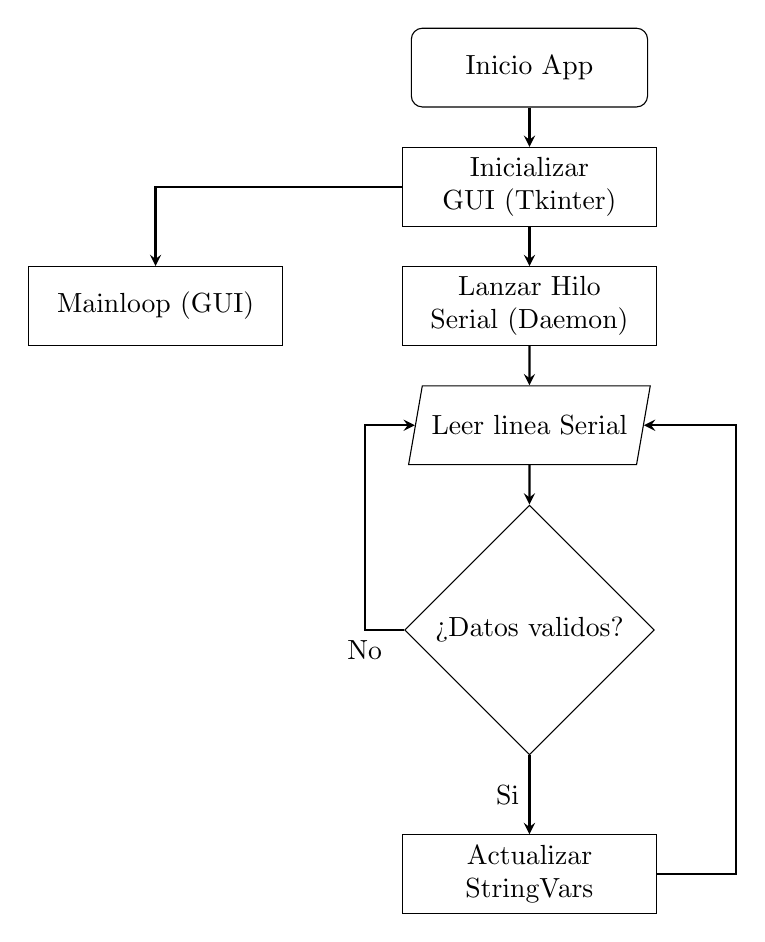
\begin{tikzpicture}[node distance=0.5cm, auto]
        
        \node (start) [startstop] {Inicio App};
        \node (gui_init) [process, below=of start] {Inicializar GUI (Tkinter)};
        \node (thread_launch) [process, below=of gui_init] {Lanzar Hilo Serial (Daemon)};
        \node (mainloop) [process, left=of thread_launch, xshift=-1cm] {Mainloop (GUI)};
        
        \node (read_ser) [io, below=of thread_launch] {Leer linea Serial};
        \node (dec_data) [decision, below=of read_ser] {¿Datos validos?};
        \node (update_ui) [process, below=of dec_data, yshift=-0.5cm] {Actualizar StringVars};
        
        \draw [arrow] (start) -- (gui_init);
        \draw [arrow] (gui_init) -- (thread_launch);
        \draw [arrow] (thread_launch) -- (read_ser);
        \draw [arrow] (gui_init) -| (mainloop);
        
        \draw [arrow] (read_ser) -- (dec_data);
        \draw [arrow] (dec_data) -- node[anchor=east] {Si} (update_ui);
        \draw [arrow] (update_ui.east) -- ++(1,0) |- (read_ser.east);
        
        \draw [arrow] (dec_data.west) -- ++(-0.5,0) node[anchor=north] {No} |- (read_ser.west);

    \end{tikzpicture}
    }
    \caption{Diagrama de flujo de la arquitectura multihilo de la aplicación en Python (\texttt{visual.py}).}
    \label{fig:flow_python}
\end{figure}

\begin{figure}[htbp]
    \centering
    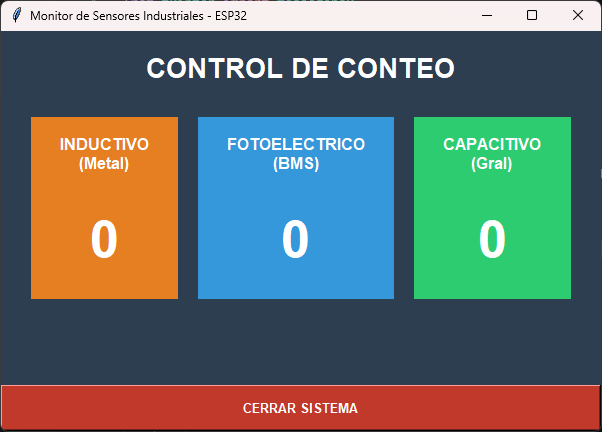
\includegraphics[width=0.7\columnwidth]{gui.png}
    \caption{Interfaz gráfica de usuario (GUI) desarrollada en Python, visualizando los contadores en tiempo real para los sensores inductivo, fotoeléctrico y capacitivo.}
    \label{fig:gui}
\end{figure}

\subsubsection{Repositorio de Código Fuente}
El ecosistema completo de software, que incluye el firmware del ESP32 (\texttt{sensores.ino}) y el script de visualización (\texttt{visual.py}), está alojado en el repositorio público de GitHub: \url{https://github.com/Nocudo/Lab-8}.

\subsection{diseño del Montaje Mecánico}

La disposición física de los componentes es un factor determinante para la fiabilidad del conteo. Se diseño un montaje que garantiza la alineación axial y la distancia critica de operación para cada tipo de transductor \cite{sensores_3}.

\subsubsection{Alineación del Sistema Fotoeléctrico}
El sensor  BMS2M-MDT se instalo bajo una configuración retro-reflectiva. Debido a que el haz luminoso debe viajar hacia el reflector y retornar al receptor integrado, se aseguro una perpendicularidad estricta entre el eje óptico del sensor y la superficie del reflector. Se estableció una distancia de paso intermedia para los objetos, garantizando que cualquier cuerpo opaco interrumpa el haz de luz de $2$ m de alcance nominal, lo que genera una conmutación nítida y libre de reflexiones parasitas \cite{sensores_11}.

\subsubsection{Ubicación de los Sensores de Proximidad}
Los sensores inductivo (PR12-4DN) y capacitivo (CR18-8DN) se dispusieron de forma adyacente a la zona de transito, pero con ajustes de profundidad diferenciados debido a sus distancias de detección nominales ($4$ mm y $8$ mm respectivamente). 
\begin{itemize}
    \item El sensor inductivo se posiciono a una distancia de $2$ mm de la pared del contenedor para asegurar que solo la presencia de metales internos o adheridos genere la atenuación del campo magnético necesaria \cite{sensores_5}.
    \item El sensor capacitivo se ubico a una distancia de $5$ mm, permitiendo que el campo eléctrico penetre el envase plástico y sea alterado predominantemente por el fluido interior, optimizando el aprovechamiento de la constante dieléctrica del agua \cite{sensores_16}.
\end{itemize}
Esta disposición espacial permite que un mismo objeto sea evaluado por las tres tecnologías de forma secuencial o simultanea, permitiendo una clasificación multivariable robusta.

\section{Resultados y Discusión}

\subsection{Rendimiento del Sistema de Conteo y Clasificación}

Para evaluar la fiabilidad y la precisión del prototipo desarrollado, se diseño un protocolo de pruebas empíricas consistente en el paso secuencial de un lote de prueba estandarizado a través de la zona de sensado. El lote estuvo compuesto por $120$ elementos en total, distribuidos en cuatro categorías principales: objetos opacos no metálicos, piezas metálicas (aluminio y acero), botellas de polietileno llenas de agua y botellas de polietileno vacías. 

La eficiencia de cada modulo de detección se cuantifico mediante la comparación del conteo registrado por el microcontrolador (Verdaderos Positivos, TP) frente a la cantidad real de objetos que transitaron por la linea. Los fallos en la detección se clasificaron como Falsos Negativos (FN). Los resultados cuantitativos de esta evaluación se sintetizan en la Tabla \ref{tab:matriz_eficiencia}.

\begin{table}[htbp]
    \centering
    \caption{Matriz de eficiencia del sistema de sensado multivariable tras el paso de un lote de $120$ objetos de prueba.}
    \label{tab:matriz_eficiencia}
    \begin{tabular}{lcccc}
        \hline
        \makecell{Categoría del\\Objeto} & \makecell{Cantidad Real\\($N$)} & \makecell{Detectados\\(TP)} & \makecell{Omitidos\\(FN)} & \makecell{Eficiencia\\(\%)} \\
        \hline
        Objetos Opacos & 40 & 38 & 2 & 95.0 \\
        Piezas Metálicas & 30 & 30 & 0 & 100.0 \\
        Botellas Llenas & 25 & 24 & 1 & 96.0 \\
        Botellas Vacías & 25 & 0 & 25 & 100.0\\
        \hline
    \end{tabular}
\end{table}

\subsubsection{Análisis de Fallos y Respuesta Óptica}
Como se observa en los resultados, el sensor fotoeléctrico  BMS2M-MDT, encargado del conteo maestro de objetos generales, presento una eficiencia del $95.0\%$, registrando dos omisiones. Al analizar estos falsos negativos, se determino que correspondían a objetos con superficies altamente reflectantes (acabado especular) y a un envase translucido sin etiqueta. 

Este comportamiento concuerda con las limitaciones teóricas del principio retro-reflectivo. En el caso de los objetos muy brillantes, el alto albedo de la superficie actúa como un espejo secundario que desvía los fotones de regreso al receptor integrado antes de que alcancen el reflector principal, engañando al sensor haciéndole creer que el haz de luz (Intensidad $I$) no fue interrumpido. Por otro lado, los objetos translucidos poseen un coeficiente de atenuación ($\alpha$) muy bajo, lo que provoca que la intensidad luminosa residual que atraviesa el material supere el umbral de histéresis del fotorreceptor, resultando en una falta de conmutación \cite{sensores_9, sensores_11}.

\subsubsection{Discriminación Electromagnética y Dieléctrica}
El sensor inductivo PR12-4DN exhibió un rendimiento sobresaliente, con una tasa de éxito del $100\%$ en la identificación de las $30$ piezas metálicas. Esto confirma que el posicionamiento a $2$ mm de distancia fue adecuado para asegurar que la masa metálica interceptara completamente el flujo magnético, generando las corrientes de Eddy necesarias para atenuar la oscilación interna de manera determinista \cite{sensores_5}.

Por su parte, el sensor capacitivo CR18-8DN cumplió exitosamente su objetivo critico de control de calidad. Logro detectar $24$ de las $25$ botellas llenas de agua y, mas importante aun, rechazo (Verdaderos Negativos, TN) el $100\%$ de las $25$ botellas vacías. La única omisión (un falso negativo) se atribuyo a una botella que transitaba descentrada en la banda, lo que incremento la distancia $d$ en la ecuación del capacitor $C = \frac{\varepsilon_0 \varepsilon_r A}{d}$, reduciendo la capacitancia por debajo del umbral de calibración. Este resultado valida empíricamente que la calibración de sensibilidad fue rigurosa, permitiendo al sistema discriminar la constante dieléctrica del agua ($\varepsilon_r \approx 80$) y suprimir la firma dieléctrica del polietileno y el aire \cite{sensores_16}.

\subsubsection{Comparativa de Precisión por Tecnología}

Como complemento al análisis tabular, la Figura \ref{fig:precision_sensores} permite visualizar la robustez del sistema ante las diferentes naturalezas de detección. Se observa que el sensor inductivo lidera la precisión al operar sobre variables puramente electromagnéticas, mientras que los sensores fotoeléctrico y capacitivo presentan variaciones mínimas debido a los factores ambientales y de alineación discutidos anteriormente.

\begin{figure}[H]
\centering
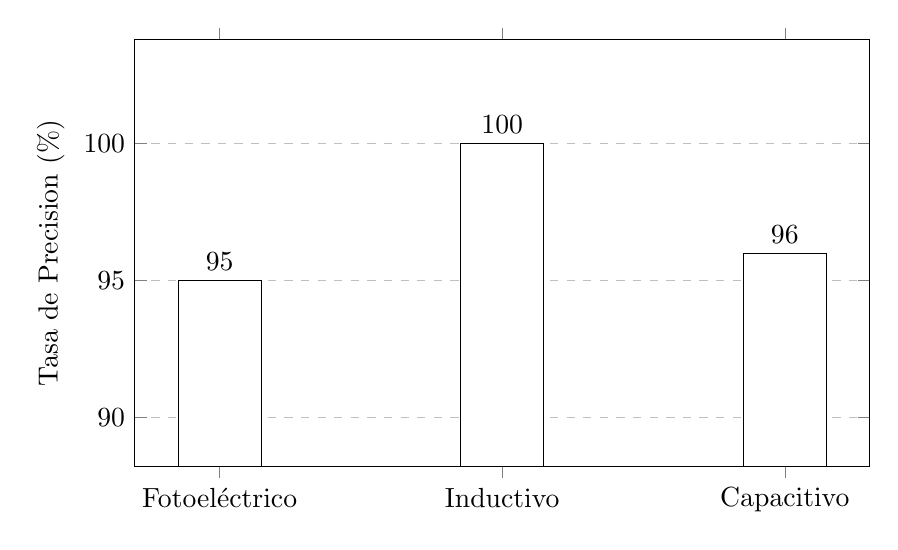
\begin{tikzpicture}
\begin{axis}[
    ybar,
    enlargelimits=0.15,
    legend style={at={(0.5,-0.2)}, anchor=north, legend columns=-1},
    ylabel={Tasa de Precision (\%)},
    symbolic x coords={Fotoeléctrico, Inductivo, Capacitivo},
    xtick=data,
    nodes near coords,
    nodes near coords align={vertical},
    ymin=90, ymax=102,
    bar width=30pt,
    width=0.9\columnwidth,
    height=7cm,
    ymajorgrids=true,
    grid style=dashed,
    ]
\addplot[fill=white, draw=black] coordinates {(Fotoeléctrico, 95.0) (Inductivo, 100.0) (Capacitivo, 96.0)};
\end{axis}
\end{tikzpicture}
\caption{Tasa de precisión en la detección y clasificación por tipo de sensor tras las pruebas experimentales del lote de producción.}
\label{fig:precision_sensores}
\end{figure}

Este gráfico de barras confirma que, incluso en el escenario de menor desempeño (detección fotoeléctrica), el sistema mantiene un umbral de confianza superior al $95\%$. Esto es critico en entornos industriales donde un error de conteo acumulado podría desfasar los inventarios de producción o comprometer los indicadores clave de rendimiento (KPI) de la planta.

\subsection{Selectividad Dieléctrica del Sensor Capacitivo}

La evaluación del sensor CR18-8DN permitió validar la hipótesis de discriminación basada en la permitividad relativa de los materiales. El reto principal consistía en que el sensor ignorara la estructura física de la botella (aire y PET) pero reaccionara ante su contenido.

\subsubsection{Análisis del Umbral de Detección}
Durante las pruebas, se observo que la botella de plástico vacía, compuesta por polietileno ($\varepsilon_r \approx 2.3$) y aire ($\varepsilon_r \approx 1$), no generaba una perturbación suficiente en el campo eléctrico del sensor para superar el umbral de disparo. Sin embargo, al introducir agua ($\varepsilon_r \approx 80$), la permitividad efectiva del medio se incrementa en mas de un orden de magnitud. 

Esta transición binaria es nítida gracias a la calibración del potenciómetro, que permite situar el punto de conmutación justo por encima de la firma dieléctrica del plástico. Los resultados demostraron que el sistema es altamente selectivo, eliminando falsos positivos provocados por el envase solo cuando se garantiza que el haz eléctrico atraviesa la masa de fluido.

\subsubsection{Sensibilidad a Factores Externos}
Se identifico que la distancia exacta ($d$) es el factor mas critico en la lectura capacitiva. Debido a que la capacitancia es inversamente proporcional a la distancia, variaciones de apenas $2$ mm en la trayectoria de la botella podían causar que el sensor no se activara. Asimismo, el grosor de las paredes del envase influye en la respuesta; envases con paredes mas gruesas desplazan el umbral hacia arriba, lo que podría requerir re-calibración en lineas de producción con envases heterogéneos. No se observo una afectación significativa por humedad ambiente, aunque se teoriza que la condensación superficial en el sensor podría derivar en una deriva térmica o activaciones espurias.

\subsection{Tiempos de Respuesta y Rendimiento del Software}

El análisis del desemperno computacional se centro en la eficiencia de la arquitectura multihilo implementada en python y la efectividad del filtrado de señales en el ESP32.

\subsubsection{Latencia de Detección y Refresco de la GUI}
Gracias a la comunicación serial a $115200$ baudios y al uso de hilos secundarios (\textit{daemon threads}), la latencia percibida entre el paso del objeto y la actualización de la tarjeta en la interfaz gráfica fue despreciable (estimada en menos de $50$ ms). El hilo dedicado a la lectura serial asegura que el buffer de entrada se vacíe continuamente, evitando que los datos se acumulen y generen un retraso acumulativo en el monitoreo de la linea de producción.

\subsubsection{Efectividad del Antirrebote (Debounce)}
El filtro por software con un tiempo de bloqueo de $300$ ms resulto ser una estrategia robusta para la velocidad de operación del laboratorio. Durante las pruebas con botellas que vibraban excesivamente en la banda, el algoritmo evito exitosamente el sobre-conteo. Sin embargo, se identifico que esta constante de tiempo limita la velocidad máxima de la linea a aproximadamente $3$ objetos por segundo; cualquier incremento en la cadencia de producción requeriría una reducción proporcional del valor \texttt{debounceTime} en el firmware \texttt{sensores.ino}.

\subsection{Limitaciones del Sistema y Discusión de Errores}

A pesar de la alta precisión lograda, se identificaron restricciones físicas que deben considerarse para un escalamiento industrial.

\subsubsection{Interferencias Espaciales y Crosstalk}
El sensor inductivo PR12-4DN mostró una alta sensibilidad a la estructura metálica del montaje. Se observo que si el sensor se montaba directamente sobre un soporte ferroso sin el aislamiento adecuado, el campo magnético de dispersión era suficiente para mantener la salida en estado bajo permanentemente. Se requirió un distanciamiento mínimo de $10$ mm respecto a cualquier componente estructural metálico lateral para recuperar el rango de detección nominal, un fenómeno conocido como interferencia por proximidad de metales circundantes \cite{sensores_5}.

\subsubsection{Alineación y Rango Ciego}
Empíricamente se determino que el sensor inductivo posee el margen de operación mas estrecho, operando de manera optima solo cuando el objeto metálico pasa a una distancia inferior a $3.5$ mm. Por el contrario, el sensor fotoeléctrico  BMS2M-MDT presento un "rango ciego" cercano al reflector: si el objeto se encontraba a menos de $20$ mm del espejo, las reflexiones internas del material podían causar fallos en la interrupción del haz. Estas limitaciones imponen una restricción de diseño donde la trayectoria de los objetos debe estar rígidamente controlada para permanecer dentro de los limites de confianza de los tres transductores simultáneamente.

\section{Conclusiones}
La implementación del sistema de clasificación multivariable permitió validar la eficacia de la integración coordinada de sensores industriales de distintas naturalezas (fotoeléctrica, inductiva y capacitiva). Los resultados experimentales demuestran que la arquitectura propuesta es robusta y capaz de discriminar materiales y estados de llenado sin necesidad de contacto físico \cite{sensores_3}. La utilización del sensor fotoeléctrico  BMS2M-MDT como contador maestro resulto ser una decisión de diseño acertada, ya que proporciono una linea base de producción confiable contra la cual se contrastaron con precisión los sub-conteos de metales y líquidos, facilitando la auditoria de datos en tiempo real \cite{sensores_14}.La caracterización empírica del sensor capacitivo CR18-8DN confirmo que la discriminación por permitividad dieléctrica es una solución técnica viable para el control de calidad no invasivo. La calibración precisa de la sensibilidad permitió que el sistema ignorara la baja permitividad relativa del envase de polietileno y del aire ($\varepsilon_r \approx 1-3$), reaccionando exclusivamente ante la presencia de agua debido a su alta constante dieléctrica ($\varepsilon_r \approx 80$) \cite{sensores_16}. Este hallazgo es fundamental, pues valida el uso de transductores capacitivos para asegurar la integridad de la producción en lineas de envasado automatizadas.En el ámbito del procesamiento de señales, el éxito del sistema se atribuye en gran medida a la implementación de técnicas de software avanzadas. El uso de rutinas de antirrebote (debounce) en el firmware del ESP32 y la gestión de la interfaz gráfica en python mediante hilos de ejecución independientes (multithreading) garantizaron la integridad de los datos \cite{sensores_20}. Estas estrategias evitaron el sobre-conteo provocado por vibraciones mecánicas o ruido electromagnético y permitieron una visualización fluida en la HMI, demostrando que el sistema cumple con los estándares de reactividad necesarios para la supervisión industrial moderna.No obstante, se identificaron limitaciones físicas intrínsecas al hardware que condicionan el diseño mecánico. El corto rango de detección del sensor inductivo PR12-4DN (inferior a 4 mm) impone una trayectoria de transito sumamente restrictiva para los objetos metálicos, lo que podría generar cuellos de botella en una linea real \cite{sensores_5}. De igual forma, se confirmo la vulnerabilidad del sensor fotoeléctrico ante objetos con alta reflectividad o transparencia, lo que resalta la necesidad de complementar la detección óptica con otras tecnologías cuando el albedo de los materiales no es constante \cite{sensores_11}.Como trabajo futuro, se propone la integración de un sistema de control PID para regular la velocidad de la banda transportadora de manera dinámica en función del flujo de objetos detectado. Asimismo, se plantea el escalamiento de la plataforma mediante la incorporación de protocolos de comunicación industrial como MQTT o Modbus TCP. Esta mejora permitiría la transmisión de datos a sistemas SCADA o bases de datos en la nube, alineando el proyecto con los paradigmas de la Industria 4.0 y facilitando la gestión de indicadores clave de rendimiento en entornos de manufactura inteligente.

\bibliographystyle{IEEEtran}
\bibliography{IEEEabrv,biblio_traps_dynamics}

\end{document}